\paragraph{Incremental Forward Stagewise Regression}
\subparagraph{Incremental Forward Stagewise Regression - $FS_{\epsilon}$}
\begin{enumerate}
	\item Start with the residual $\bm{r}$ equal to $\bm{y}$ and $\beta_{1}, \beta_{2}, \cdots,
		\beta_{p}$ = 0. All the predictors are standardized to have mean zero and unit norm.
	\item Find the predictor \sB{$x_{j}$ most correlated with $\bm{r}$}
	\item Update \sB{$\beta_{j} \leftarrow \beta_{j} + \delta_{j}$}, where \tB{$\delta_{j} = 
		\epsilon\times \text{sign}[\sP{\bm{x}_{j}}{\bm{r}}]$} and $\epsilon>0$ is a small
		step size, and set \sB{$\bm{r} \leftarrow \bm{r} - \delta_{j}\bm{x}_{j}$}
	\item Repeat steps 2 and 3 many times, until the residuals are uncorrelated with all the
		predictors.
\end{enumerate}

The linear regression version of the forward-stagewise generates a coefficient profile by
repeatedly updating (by a small amount $\epsilon$ the coefficient of the variable most correlated
with the current residual.\\
If $\delta_{j}= \sP{\bm{x}_{j}}{\bm{r}}$ (the least squares coefficient of the residual on $j^{th}$
predictor), then this is exactly the usual forward stagewise procedure (FS).\\
Letting $\epsilon \rightarrow 0$ gives the right panel, which in this case is identical to the lasso
path. We call this limiting procedure infinitesimal forward stagewise regression or $FS_{0}$
\begin{figure}[H]
	\begin{center}
		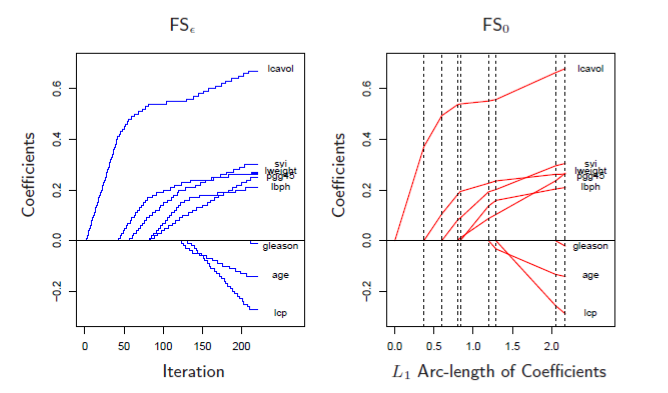
\includegraphics[width=.7\textwidth]{chap/1chap/5sec/images/7_coefficientsFS.PNG}
	\end{center}
	\caption{The left pannel shows incremental \tB{forward stagewise regression with step size
	$\epsilon=0.01$}. The right panel shows the infinitesimal version \tB{$FS_{0}$ obtained 
	letting $\epsilon \rightarrow 0$}}
	\label{fig:7_coefficientsFS}
\end{figure}

\subparagraph{Least Angle Regression $FS_{0}$}
\begin{itemize}
	\item[4] Find the new direction by solving the constrained least squares problem:
		\begin{center}
		\encN{
		$\min\limits_{b}\norm{\bm{r}-\bm{X}_{\mathcal{A}}b}^{2}_{2} \text{subject to }
		b_{j}s_{j}\geq0, j\in\mathcal{A}$}
		\end{center}
		where $s_{j}$ is the sign of $\sP{\bm{x}_{j}}{
		\bm{r}}$
\end{itemize}
While the Lasso makes optimal progress in terms of reducing the residual sum-of-squares per unit
increase in $L_{1}$-norm of the coefficient vector $\beta$. $FS_{0}$ is optimal per unit increase
in $L_{1}$ arc-length traveled along the coefficient path. Hence \sB{its coefficient path is 
discouraged from changing direction too often}.

\paragraph{Piecewise-Linear Path Algorithms}
\begin{center}
\encB{$\hat{\bm{\beta}}(\lambda) = \min\limits_{\beta}\left( \bm{R}(\beta) + \lambda\bm{J}(\beta) 
\right) \text{with} \bm{R}(\beta) = \su{{i=1}}{N}\bm{L}\left( y_{i}, \beta_{0}+\su{{j=1}}{p}x_{ij}
\beta_{j}\right)$}
\end{center}
with both the loss function $\bm{L}$ and the \sB{penalty function $\bm{J}$} are convex.\\
Then the following are sufficient conditions for the solution path $\beta(\lambda)$ to be piecewise
linear.
\begin{enumerate}
	\item $R$ is quadratic or piecewise-quadratic as a function of $\beta$
	\item $J$ is a piecewise linear in $\beta$
\end{enumerate}

\paragraph{The Dantzig Selector}
\begin{center}
\encB{$\min\limits_{\beta}\norm{\bm{X}^{T}\left( \bm{y}-\bm{X}\beta \right)}_{\infty} \text{subject
to } \norm{\beta}_{1}$}
\end{center}
Here $\norm{.}_{\infty}$ denotes the $L_{\infty}$ norm, the maximum absolute 
value of the components of the vector.

\paragraph{The Grouped Lasso}
Suppose that the $p$ predictors are divised in $L$ groups, with \sB{$p_{l}$ the number in group $l$}.
\\
\sB{$\bm{X}_{l}$ represents the predictors corresponding to the $l^{th}$ group}, with corresponding 
coefficient vector $\beta_{l}$.\\
The grouped-lasso minimizes the convex criterion
\begin{center}
\encB{$ \min\limits_{\beta\in\mathbb{R}^{p}}\left( \norm{\bm{y}-\beta_{0}\bm{1}-\su{{l=1}}{L}\bm{X}_{
l}\beta_{l}}^{2}_{2} + \lambda\su{{l=1}}{L}\sqrt{p_{l}}\norm{\beta_{l}}_{2} \right)$}
\end{center}
where \sB{the $\sqrt{p_{l}}$ terms accounts for the varying group sizes}, $\norm{.}_{2}$ is the 
Euclidean norm (not squared). Since the Euclidean norm of a vector $\beta_{l}$ is zero only if all 
its components are zero, this procedure encourages sparsity at both the group and individual levels.
